% !TEX root = main.tex
% =============================================================================
% Problem formulation
% =============================================================================

\section{Problem Formulation}
\label{sec:problem}

\subsection{Setting}
\label{sec:problem:setting}

The geometric refine starts after a discrete multi-group router has returned a
feasible coarse layout.
We treat the following as \emph{fixed}:

\begin{itemize}
  \item \textbf{Domain} $\Omega$: a bounded design region with static obstacles
        and already committed pipes of other groups (permanent clearance).
  \item \textbf{Topology} $\mathcal{T}$: for each group, a connected graph
        (typically a tree), together with a feasible coarse polyline or grid
        embedding that initializes the refine.
  \item \textbf{Usages} $\mathcal{U}$: a set of directed terminal--terminal
        flows that must be considered when scoring fairness
        (e.g.\ $A\!\to\!C$, $B\!\to\!C$, $A\!\to\!B$).
  \item \textbf{Radii and ports}: tube radii along the layout, fixed terminal
        positions, and optional end-tangent / line-axis clamps so that a port
        sits on a prescribed axis.
\end{itemize}

The decision variables $X$ parameterize centerlines (and, implicitly,
tubular solids of the given radii).
The output must keep every terminal connected as in $\mathcal{T}$: each declared
usage remains a continuous path between its ends.
Branches need not meet at a single geometric point; Sec.~\ref{sec:problem:junction}
explains when a local split near a junction is allowed.

\subsection{Objective sketch}
\label{sec:problem:objective}

Given topology $\mathcal{T}$ and a feasible coarse embedding, refine the
geometric parameters $X$ so that a weighted soft cost over declared usages is
minimized, subject to hard geometric constraints:
\begin{equation}
\label{eq:stage1}
\min_{X}
\;
J_{\mathrm{path}}(X)
+
J_{\mathrm{clear}}(X)
+
J_{\mathrm{union}}(X)
+
J_{\mathrm{space}}(X)
\quad
\text{s.t.\ ports, }\mathcal{T}\text{, interface }C^{0}/C^{1}
\text{ by construction.}
\end{equation}
Table~\ref{tab:soft-hard} summarizes the roles of the terms.
Full discrete definitions appear in Sec.~\ref{sec:costs}; here we only fix the
semantics needed for the problem statement.

\begin{table}[H]
  \centering
  \caption{Soft versus hard elements in the geometric refine.}
  \label{tab:soft-hard}
  \begin{tabular}{@{}p{0.22\linewidth}p{0.48\linewidth}p{0.22\linewidth}@{}}
    \toprule
    Symbol & Role & Soft / hard \\
    \midrule
    $X$
      & Centerline parameters (shared trunk + private junction controls)
      & decision \\
    $L,K$ in $J_{\mathrm{path}}$
      & Chord energy (each shared piece once) + bend (segment interiors once;
        usage joints once)
      & soft \\
    $J_{\mathrm{clear}}$
      & Obstacle and cross-group tube separation
      & soft in loop; \textbf{hard} at accept \\
    $J_{\mathrm{union}}$
      & Junction-bundle compactness
      & soft \\
    $J_{\mathrm{space}}$
      & Keep sample gaps comparable under parameter sampling
      & soft \\
    Topology / ports / interface
      & Connectivity, fixed ends, $C^{0}/C^{1}$ clamps
      & \textbf{hard} (by construction) \\
    \bottomrule
  \end{tabular}
\end{table}

\subsection{Difference from classical path smoothing}
\label{sec:problem:diff}

\begin{table}[H]
  \centering
  \caption{Classical path smoothing versus the pipe refine studied here.}
  \label{tab:vs-smooth}
  \begin{tabular}{@{}p{0.22\linewidth}p{0.34\linewidth}p{0.34\linewidth}@{}}
    \toprule
    Aspect & Normal path smoothing & This problem \\
    \midrule
    Occupancy
      & Pass-and-release (time / moving agent)
      & Permanent tubes; clearance is static geometry \\
    Structure
      & Single $s$--$t$ line
      & Tree / branched manifold; degree $\ge 3$ joins \\
    Cost scope
      & One path's length / curvature
      & Usage-assembled paths over the branched manifold \\
    Domain
      & Often open or mild
      & Tight $\Omega$ may force large $\kappa$ (soft $K$) \\
    Ends
      & Fixed $s,t$ (pose optional)
      & Fixed ports plus line-axis alignment \\
    \bottomrule
  \end{tabular}
\end{table}

\subsection{Junction conflict: shared node versus local split}
\label{sec:problem:junction}

Usages matter because shared trunk nodes couple directions.
Optimizing only the shared polyline can make $A\!\to\!C$ and $B\!\to\!C$ smooth
while $A\!\to\!B$ remains a hairpin at the branch.
The declared set $\mathcal{U}$ therefore decides which end-to-end paths must stay
fair, and where junctions need private degrees of freedom.

Consider a Y-junction with fixed topology and usages
$\mathcal{U}=\{A\!\to\!C,\, B\!\to\!C,\, A\!\to\!B\}$:
\[
A\text{---}J\text{---}C,\qquad B\text{---}J.
\]

\paragraph{Shared junction.}
All three branches meet at one point $J$.
Fair geometry for $A\!\to\!C$ and $B\!\to\!C$ forces a sharp turn on
$A\!\to\!B$ at $J$ (Fig.~\ref{fig:y-shape}a).

\paragraph{Locally split junction.}
Private junction degrees of freedom let $A\!\to\!B$ take a dedicated arc while
$A\!\to\!C$ and $B\!\to\!C$ keep a shared trunk (Fig.~\ref{fig:y-shape}b).
A void appears near the join; connectivity of $\mathcal{T}$ is preserved, but
the embedding need not keep a common junction point.

\begin{figure}[H]
  \centering
  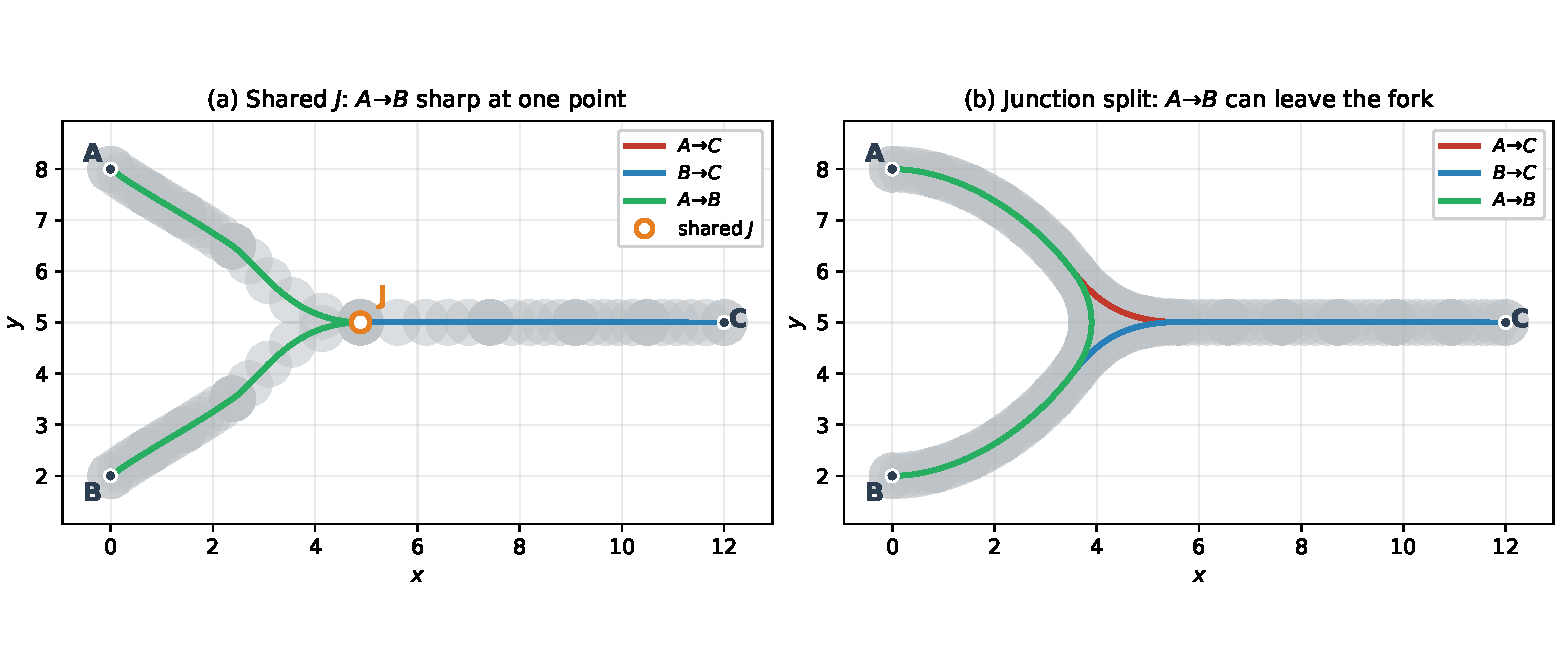
\includegraphics[width=\linewidth]{figures/y_shape_shared_vs_split.pdf}
  \caption{Planar Y under the same usages
  $\mathcal{U}=\{A\!\to\!C,\,B\!\to\!C,\,A\!\to\!B\}$ (top view; gray disks =
  tube radius).
  (a)~Forced shared connect point: the three usage centerlines meet at one
  node $J$ (orange); refine can fair $A\!\to\!C$ and $B\!\to\!C$, but
  $A\!\to\!B$ (green) stays sharp at $J$.
  (b)~Hybrid trunk-share / junction-split: $A\!\to\!B$ can leave the fork
  while the trunk toward $C$ remains shared.}
  \label{fig:y-shape}
\end{figure}

\begin{table}[H]
  \centering
  \caption{Shared junction versus locally split junction.}
  \label{tab:junction-regimes}
  \begin{tabular}{@{}lll@{}}
    \toprule
    & Shared junction & Locally split junction \\
    \midrule
    Geometry at join
      & one shared point $J$
      & trunks + dedicated $A\!\to\!B$ arc + void \\
    $A\!\to\!C$, $B\!\to\!C$
      & arc + straight
      & same as shared case \\
    $A\!\to\!B$
      & sharp at $J$
      & dedicated arc; fair \\
    $\mathcal{T}$
      & preserved
      & preserved (connectivity, not a common join point) \\
    \bottomrule
  \end{tabular}
\end{table}

The design implication is that the refine must allow private degrees of freedom
near junctions (local split) while sharing trunk controls where usages truly share
physical pipe.
That hybrid structure---trunk-share + junction-split---is the method focus of
this report.
The core gap relative to single-curve fairing is therefore
\textbf{topology-preserving, multi-usage geometric refinement under permanent
tubular occupancy}, not merely denser spline fitting.

\subsection{Place in the pipeline}
\label{sec:problem:pipeline}

A typical valve-channel workflow is discrete multi-group routing, then
centerline refine, then CAD solids, then fluid PDE / shape polish.
This report covers only the geometric refine.

That ordering matters for junctions.
Downstream shape or adjoint PDE optimization usually deforms a
\emph{fixed} channel layout: it can move walls or a shared centerline, but it
does not introduce a new split curve or triangular void at a Y-join the way
a locally split junction does.
That local split is therefore a decision of the geometric refine, not of
later physics polish.
We still preserve the connectivity of $\mathcal{T}$ (no discrete rewiring);
what changes is the geometric arrangement near degree-$\ge 3$ nodes.
Pressure drop and streamline quality remain for subsequent physics-based
optimization, once the centerline graph---including any local splits---is
fixed.
